% Plantilla común para figuras redibujadas (fig-NN-desc.tex).
% Copiar entera y sustituir solo el cuerpo entre las marcas "cuerpo de la figura".
% Compila tal cual en Overleaf o con scripts/tikz2svg.sh.
%
% NO añadir la opción "tikz" a standalone: parte cada tikzpicture (y cada
% \chemfig) en una página distinta y el SVG solo tendría la primera.
\documentclass[border=4pt]{standalone}
\usepackage[T1]{fontenc}
\usepackage{lmodern}            % base vectorial: sin fuente vectorial el texto sale en Type 3 y dvisvgm lo pierde
\usepackage[scaled=0.95]{helvet}% sans-serif tipo Helvetica, como la interfaz de Obsidian
\renewcommand{\familydefault}{\sfdefault}
\usepackage{amsmath,amssymb}
\usepackage{sansmath}\sansmath  % fórmulas en sans, a juego con el texto
\usepackage[version=4]{mhchem}  % \ce{A + B -> C}
\usepackage{chemfig}            % estructuras y esquemas de reacción
\usepackage{tikz}
\usetikzlibrary{arrows.meta,positioning,calc,shapes.geometric,decorations.pathmorphing,decorations.markings}
\usepackage{pgfplots}           % gráficas (cinética, curvas de valoración...)
\pgfplotsset{compat=1.18}

% ---- Estilo Apuntes.md --------------------------------------------------
% Paleta semántica (la misma que el CSS de Obsidian). Principios inspirados en
% figures4papers (ChenLiu-1996, CC BY-NC 4.0): se adoptan ideas, no código.
\definecolor{apAzul}{HTML}{0F4D92}       % anotaciones, estructura (el azul del autor)
\definecolor{apAzulClaro}{HTML}{3775BA}
\definecolor{apRojo}{HTML}{B64342}       % curvas y datos principales, importante (el rojo del autor)
\definecolor{apRojoClaro}{HTML}{E9A6A1}
\definecolor{apVerde}{HTML}{3B7D3B}      % definiciones, "positivo"
\definecolor{apVerdeClaro}{HTML}{AADCA9}
\definecolor{apGris}{HTML}{767676}       % apoyo: rejillas, referencias, líneas punteadas
\definecolor{apGrisClaro}{HTML}{CFCECE}
\definecolor{apNegro}{HTML}{272727}      % ejes y texto neutro

\tikzset{
  % sin "color=" global: pisaría los \color{...} de chemfig (estructuras en rojo, etc.)
  every picture/.append style={line width=0.9pt, >={Stealth[length=2.4mm]}},
  curva/.style={apRojo, line width=1.6pt},                  % la curva o el dato que importa
  curva secundaria/.style={apAzulClaro, line width=1.3pt},
  referencia/.style={apGris, dotted, line width=1pt},       % líneas guía (p. ej. y = 0)
  anotacion/.style={apAzul, font=\normalsize},              % texto escrito a mano alrededor del dibujo
  flecha/.style={->, apAzul, line width=1pt},
  implica/.style={-{Implies}, double, double distance=2pt, line width=0.8pt},
  marca/.style={circle, fill=apAzul, draw=white, line width=0.6pt, inner sep=1.8pt},
  resalte/.style={apAzul, line width=1pt},                  % círculos/óvalos que rodean algo
}
\pgfplotsset{
  apuntes/.style={
    axis lines=left, axis line style={line width=1pt, apNegro, -{Stealth[length=2.4mm]}},
    tick style={apNegro, line width=0.8pt}, tick align=outside,
    label style={font=\normalsize}, tick label style={font=\normalsize},
    every axis plot/.append style={curva},
    clip=false,
  },
}
\setchemfig{atom sep=2em, bond style={line width=0.9pt}}
% -------------------------------------------------------------------------

\begin{document}
% --- cuerpo de la figura ---
% Jerarquía a nivel submolecular y molecular (pág. 3)
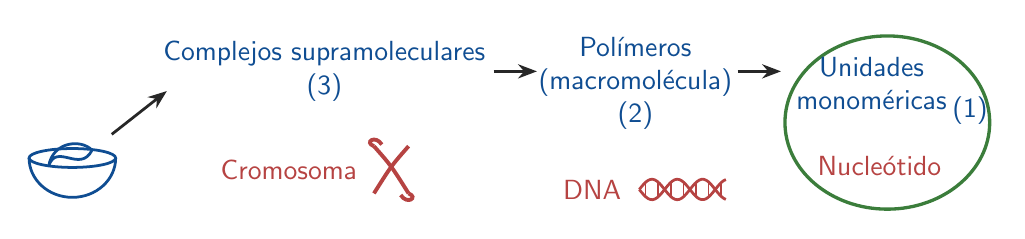
\begin{tikzpicture}[font=\normalsize]
  % "cuenco" con contenido (dibujo sin etiqueta en la hoja)
  \begin{scope}[apAzul, line width=1pt]
    \draw (-0.55,0.15) arc (180:360:0.55 and 0.5);
    \draw (0,0.15) ellipse (0.55 and 0.12);
    \draw (-0.3,0.05) .. controls (-0.2,0.35) and (0.1,-0.05) .. (0.25,0.25) .. controls (0.1,0.4) and (-0.25,0.35) .. cycle;
  \end{scope}
  \draw[flecha, apNegro] (0.5,0.45) -- (1.2,1.0);

  % (3) complejos supramoleculares -> cromosoma
  \node[anotacion, align=center] at (3.2,1.25) {Complejos supramoleculares\\(3)};
  \node[apRojo] at (2.75,0.0) {Cromosoma};
  \begin{scope}[shift={(4.05,0.0)}, apRojo, line width=1.4pt]
    \draw (-0.22,0.3) .. controls (0,0.05) .. (0.22,-0.3);
    \draw (0.22,0.3) .. controls (0,0.05) .. (-0.22,-0.3);
    \draw (-0.22,0.3) .. controls (-0.35,0.35) and (-0.2,0.45) .. (-0.12,0.32);
    \draw (0.22,-0.3) .. controls (0.35,-0.35) and (0.2,-0.45) .. (0.12,-0.32);
  \end{scope}
  \draw[->, apNegro, line width=1pt] (5.35,1.25) -- (5.9,1.25);

  % (2) polímeros -> DNA
  \node[anotacion, align=center] at (7.15,1.1) {Polímeros\\(macromolécula)\\(2)};
  \node[apRojo] at (6.6,-0.25) {DNA};
  \begin{scope}[shift={(7.2,-0.25)}, apRojo, line width=1pt]
    \draw[domain=0:1.1, samples=40, variable=\x] plot (\x, {0.13*sin(\x*560)});
    \draw[domain=0:1.1, samples=40, variable=\x] plot (\x, {-0.13*sin(\x*560)});
    \foreach \x in {0.08,0.24,...,1.05} \draw[line width=0.6pt] (\x,{0.13*sin(\x*560)}) -- (\x,{-0.13*sin(\x*560)});
  \end{scope}
  \draw[->, apNegro, line width=1pt] (8.45,1.25) -- (9.0,1.25);

  % (1) unidades monoméricas -> nucleótido, rodeado en verde
  \draw[apVerde, line width=1.2pt] (10.35,0.6) ellipse (1.3 and 1.1);
  \node[anotacion, align=center] at (10.15,1.1) {Unidades\\monoméricas};
  \node[anotacion] at (11.4,0.75) {(1)};
  \node[apRojo] at (10.25,0.05) {Nucleótido};
\end{tikzpicture}
% ---------------------------
\end{document}
